\section{Iterazione 0}
\subsection{Introduzione e panoramica del sistema}
Il sistema che verrà implementato in questo progetto di studio si occuperà della gestione di un centro di immersioni, noto anche come \emph{diving center} o \emph{dive center}. Un centro di immersione è una struttura che fornisce supporto, attrezzatura e corsi per la pratica delle attività subacquee. Un centro di immersione fornisce principalmente tre tipi di servizi:
\begin{itemize}
    \item Immersioni guidate.
    \item Noleggio attrezzatura.
    \item Scuola di immersione.
\end{itemize}
Per immersione guidata si intende un'immersione effettuata in gruppo o singolarmente insieme a guide subacquee addestrate, esperte e a conoscenza dei punti di immersione più importanti ed interessanti. Questa soluzione è ottimale quando ci si vuole immergere in luoghi non conosciuti o in parchi marini protetti per cui è necessaria un'autorizzazione e una guida. Inoltre, il centro diving offre i servizi di accompagnamento e assistenza, di trasposto con imbarcazioni o gommoni, che permettono l'entrata e l'uscita dall'acqua con praticità e comfort.
\\
Il focus del nostro progetto sarà la gestione e l'organizzazione efficiente delle immersioni guidate e la gestione del noleggio attrezzatura; non verrà incluso l'insegnamento della pratica subacquea.
\\
Un centro di immersione ha una disponibilità limitata di barche e guide per cui ha la possibilità di effettuare un numero limitato di escursioni durante una giornata. Il sistema che verrà sviluppato si occuperà di organizzare al meglio l'allocazione delle risorse disponibili affinché un numero maggiore di persone possa parteciparvi. Spesso le persone che vogliono partecipare a questo tipo di escursioni si trovano in gruppo, per cui è necessario ottimizzare l'allocazione delle risorse disponibili, che in questo caso costituiscono i posti disponibili in barca, con il vincolo di mantenere il più possibile intatti i gruppi.
\\
Il sistema implementato rappresenterà un centro di immersione: si occuperà della gestione delle risorse (barche, escursioni, attrezzatura disponibile) e della gestione delle prenotazioni delle escursioni da parte degli utenti.
\subsection{Requisiti funzionali e analisi dei casi d'uso}

In questa sezione verranno introdotti i requisiti funzionali del sistema attraverso l'utilizzo dei casi d'uso.
\\Lo schema UML dei casi d'uso viene riportato in Figura~\ref{fig:casiduso}.

\begin{figure}[htbp]
    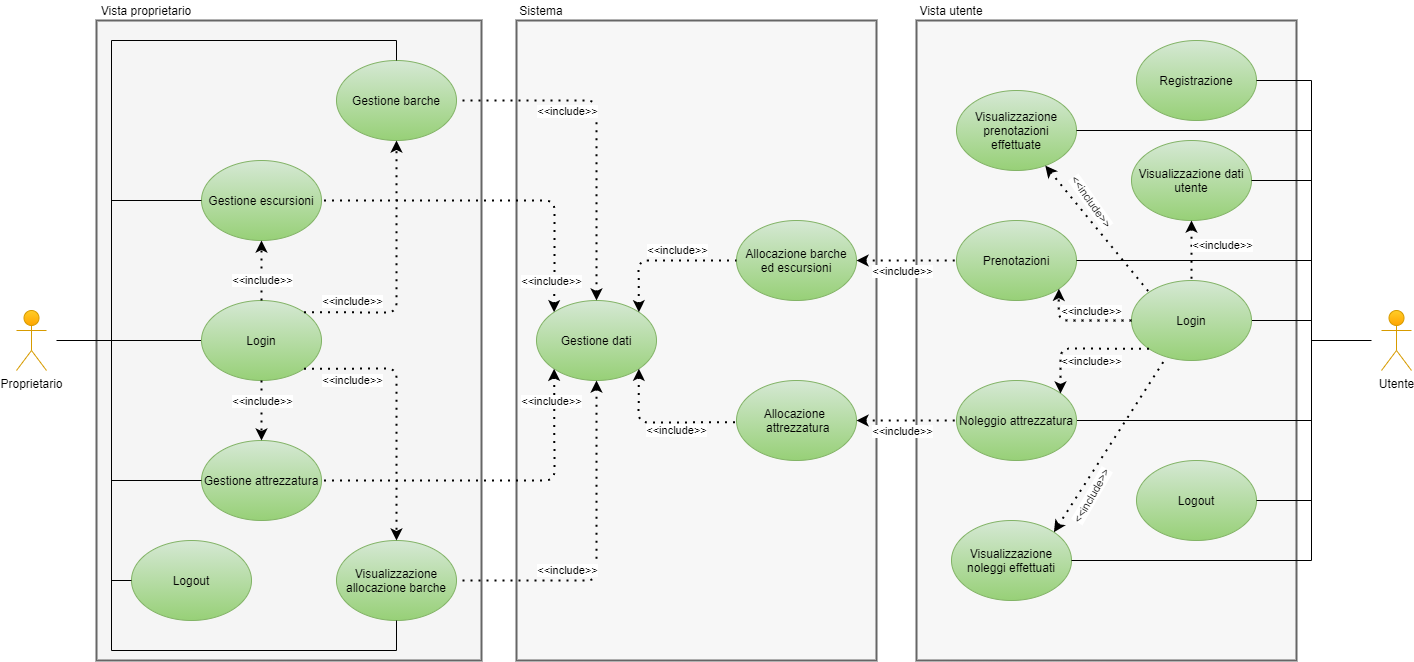
\includegraphics[width=\textwidth]{iterazione0/useCases_v6.png}
    \centering
    \caption{Diagramma UML dei casi d'uso}\label{fig:casiduso}
\end{figure}

Al fine di procedere ad uno sviluppo efficiente, è stato deciso di dividere le specifiche funzionali in tre code di priorità: alta, media e bassa. Nella coda ad alta priorità si troveranno i casi d'uso indispensabili al corretto funzionamento dell'applicazione, nella coda a media priorità saranno inserti i casi d'uso riguardanti le funzionalità aggiuntive e nella coda a bassa priorità le funzionalità non strettamente necessarie e che verranno implementate in versioni future.

\clearpage
\subsubsection{Coda ad alta priorità}

\begin{table}[htbp]
 \centering
 \begin{tabularx}{\textwidth}{|>{\centering\arraybackslash} m{4em}| >{\raggedright\arraybackslash}X |} 
 \hline
 \textbf{Codice} & \textbf{Titolo} \\ [0.5ex]
 \hline\hline
UC1 & Gestione barche (visualizzazione, inserimento, modifica, elimina) \\
\hline
UC2 & Gestione escursioni (visualizzazione, inserimento, modifica, elimina) \\
\hline
UC3 & Registrazione utente \\
\hline
UC4 & Login utente \\
\hline
UC5 & Logout utente \\
\hline
UC6 & Gestione prenotazioni (visualizzazione, inserimento) \\
\hline
UC7 & Algoritmo gestione barche ed escursioni \\
\hline
\end{tabularx}
\caption{Casi d'uso con priorità alta}
\label{Casi d'uso con priorità alta}
\end{table}

\subsubsection{Coda a media priorità}

\begin{table}[htbp]
 \centering
 \begin{tabularx}{\textwidth}{|>{\centering\arraybackslash} m{4em}| >{\raggedright\arraybackslash}X |} 
 \hline
 \textbf{Codice} & \textbf{Titolo} \\ [0.5ex] \hline\hline
UC8 & Visualizzazione allocazione barche \\
\hline
UC9 & Gestione attrezzatura (visualizzazione, inserimento, modifica, elimina) \\
\hline
UC10 & Noleggio attrezzatura \\
\hline
UC11 & Algoritmo attrezzatura \\
\hline
\end{tabularx}
\caption{Casi d'uso con priorità media}
\label{Casi d'uso con priorità media}
\end{table}

\subsubsection{Coda a bassa priorità}

\begin{table}[htbp]
 \centering
 \begin{tabularx}{\textwidth}{|>{\centering\arraybackslash} m{4em}| >{\raggedright\arraybackslash}X |} 
 \hline
 \textbf{Codice} & \textbf{Titolo} \\ [0.5ex] \hline\hline
UC12 & Visualizzazione dati utente \\
\hline
UC13 & Modifica dati utente \\
\hline
UC14 & Visualizzazione prenotazioni effettuate \\
\hline
UC15 & Visualizzazione noleggi effettuati \\
\hline
\end{tabularx}
\caption{Casi d'uso con priorità bassa}
\label{Casi d'uso con priorità bassa}
\end{table}

\clearpage

\subsection{Requisiti non funzionali}
Il progetto verrà sviluppato tenendo in considerazione anche alcuni requisiti non funzionali, quali la manutenibilità, l'efficienza e l'usabilità.
\subsubsection{Manutenibilità}
Il requisito di manutenibilità verrà rispettato mediante l'implementazione di tutte le risorse persistenti, ovvero barche, orari e date delle escursioni, attrezzatura. In questo modo, anche se in futuro dovessero cambiare alcune condizioni, sarebbe facile per il proprietario rifletterle all'interno del software.
\subsubsection{Efficienza}
Il requisito dell'efficienza è anche l'obiettivo primario del progetto, ovvero l'allocazione ottimale delle risorse disponibili: i posti presenti nelle barche.
\subsubsection{Usabilità}
L'usabilità è garantita dalla decisione di sviluppare il programma attraverso un applicazione Android, di facile utilizzo sia per gli utenti che per il proprietario. In base alla topologia (Figura~\ref{fig:topologia}) è possibile notare che il database verrà ospitato da un hosting online e quindi sarà sempre possibile, mediante cellulare, accedere a tutte le funzionalità dell'applicazione.

\newpage

\subsection{Topologia del sistema}
La topologia del sistema mostrata in Figura~\ref{fig:topologia}, evidenzia il requisito non funzionale dell'usabilità: sia gli utenti che il proprietario possono accedere al servizio tramite l'applicazione. Il WebServer espone un set di API mediante HTTP/REST con cui è possibile accedere alle funzionalità dell'applicazione. Infine, il WebServer è collegato ad un database relazionale.

Questo progetto è stato sviluppato utilizzando un’architettura \textit{Three-tier}, ovvero un’architettura hardware di tipo multi-tier. Essa prevede la suddivisione dell’applicazione in tre diversi moduli, i quali risiedono su macchine separate, dedicati rispettivamente a:
\begin{itemize}
    \item Presentation, interfaccia utente
    \item Application, logica funzionale
    \item Data, gestione dei dati persistenti.
\end{itemize}

È possibile visualizzare questa divisione in Figura \ref{fig:topologia}.

\subsection{Design pattern MVP}
Il sistema e i suoi componenti verranno sviluppati utilizzando il design pattern architetturale Model View Presenter (MVP), una derivazione del Model View Controller (MVC). MVP è composto da tre layer: \begin{itemize}
    \item Model, che definisce i dati da dell'applicazione e può essere visto come un'interfaccia responsabile di accedere alle API connesse con il database. 
    \item View, che visualizza i dati e notifica le azioni dell’utente. Solitamente non presenta nessuna logica applicativa, ma ha una funzione solo visuale. 
    \item Presenter, che contiene la logica applicativa. Funziona come man-in-the-middle tra la View e il Model, prendendo i dati dal Model e formattandoli per la View.
\end{itemize}
A differenza del MVC, la View non è direttamente collegata al Model; l'interazione può avvenire solo tramite il Presenter. Questo permette uno sviluppo indipendente dei tre livelli. Tale separazione è visibile anche nelle componenti software, come si vede in Figura \ref{fig:componentDiagram}.

\begin{figure}[htbp]
    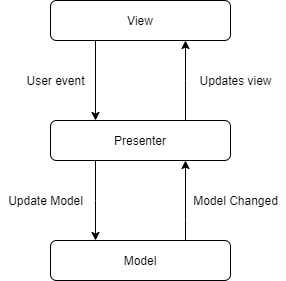
\includegraphics[width=\textwidth]{/iterazione0/MVP.png}
    \centering
    \caption{Model View Presenter}\label{fig:MVP}
\end{figure}
\begin{figure}[htbp]
    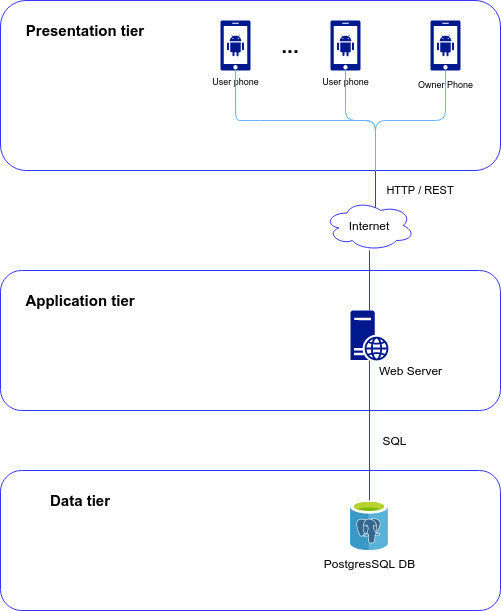
\includegraphics[width=\textwidth]{/iterazione0/topologia_v3.png}
    \centering
    \caption{Topologia del sistema}\label{fig:topologia}
\end{figure}

\clearpage
\subsection{Toolchain e tecnologie}

\subsubsection{Elenco completo}

\begin{table}[htbp]
 \centering
 \begin{tabularx}{\textwidth}{| >{\raggedright\arraybackslash}X | >{\raggedright\arraybackslash}X |} 
 \hline
 \textbf{Tool/Tecnologia} & \textbf{Utilizzo} \\ [0.5ex]
 \hline\hline
Visual Studio Code & IDE per sviluppo back-end \\
\hline
Spring Boot & Java Framework per realizzazione back-end\\
\hline
Android Studio & IDE per sviluppo front-end \\
\hline
Kotlin & Linguaggio di programmazione per realizzazione front-end \\
\hline
Git e GitHub & Software e piattaforma per versionamento e condivisione di codice e documentazione \\
\hline
Google Drive & Cloud Storage per condivisione di documenti e immagini \\
\hline
Trello & Software gestionale per schedulazione attività tra i componenti del team per sviluppo agile\\
\hline
Jupyter Notebook con Python & Ambiente per testare l'algoritmo centrale del progetto\\
\hline
Canva & Tool di progettazione grafica per presentazione dell'applicazione \\
\hline
Draw.io & Tool per realizzazione grafici e diagrammi UML \\
\hline
Language Support for Java(TM) by Red Hat & Estensione di Visual Studio Code per analisi statica del codice a back-end \\
\hline
Postman & Piattaforma per test dinamico e documentazione delle API \\
\hline
JUnit 5 & Framework per Unit Testing \\
\hline
Overleaf & Software per la stesura e formattazione della documentazione in linguaggio LaTeX \\
\hline
\end{tabularx}
\caption{Toolchain e tecnologie}
\label{Toolchain e tecnologie}
\end{table}

\subsubsection{Tecnologie per analisi statica} \label{analisi-statica}

Per l'analisi statica del codice a backend è stata utilizzata l'estensione \textit{Language Support for Java(TM) by Red Hat} fornita
dall'IDE \textit{Visual Studio Code}.
Questa permette di seguire le regole di formattazione standard di Java e avere una migliore leggibilità del codice, mantenendone
alta la qualità.

\subsubsection{Tecnologie per analisi dinamica}
Per l'analisi dinamica del codice è stato utilizzato \textit{Postman}, software che permette sia di richiamare le API realizzate a back-end, sia di testarle realizzando test dinamici.
\clearpage
